\documentclass{article}
\usepackage[utf8]{inputenc}
\usepackage{amsmath}
%to insert math symbols like implies
\usepackage{graphicx}
%to insert images,graphs
\usepackage{amssymb}


\title{ASSIGNMENT_1}
\author{AI21BTECH11021}
\date{March 2022}

\begin{document}

\maketitle

\section*{Question 3 (c)}
\begin{figure}[h!]
    \centering
    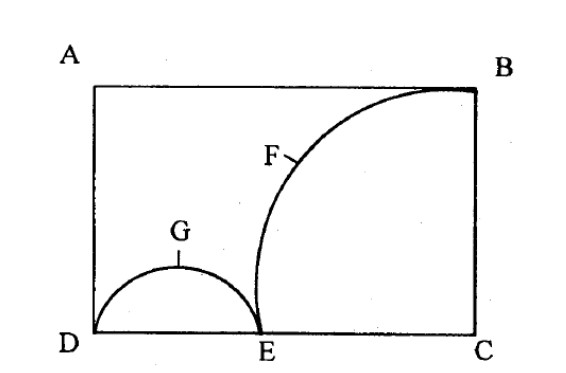
\includegraphics[scale = 0.5]{Figure_1.jpg}
    \caption{rectangle}
    \label{fig:my_label}
\end{figure}

In the figure given below, \textbf{ABCD} is a rectangle.\textbf{AB} = 14 cm\textbf{BC} = 7 cm.\\
From the rectangle, a quarter circle \textbf{BFEC} and a semicircle \textbf{DGE} are removed.\\
Calculate the area of the remaining piece of the rectangle?.\\
( Take $ \pi = 22/7 $)\\

\begin{align*}
\rule{\textwidth}{0.4pt}\\    
\end{align*}

\section*{solution:}
\begin{center}
\begin{align*}
    Area\;of\;rectangle &= length*width\\
    Area\;of\;circle &=\pi*radius^2 \\
\end{align*}
\end{center}

\begin{center}
 \begin{align*}
     so\;area\;of\;rectangle\;ABCD &= 14cm*7cm\\
                 &= 98cm^2.\\
\end{align*}
\end{center}

\begin{align*}
Area\;of\;quater\;circle &= \frac{1}{4}*\pi*(radius)^2\\
Area\;of\;\textbf{BFEC}\;region &= \frac{1}{4}*\pi*(7cm)^2\\ 
    &= \frac{77}{2}cm^2(radius\;is\;BC)\\
    \\
Area\;of\;semicircle\;&=\;\frac{1}{2}*\pi*(radius)^2\\
Area\;of\;\textbf{GD}E\;region\;&=\;\frac{1}{2}*\pi*(\frac{7}{2}cm)^2\\
    &= \frac{77}{4}cm^2 \\ \\
\end{align*}
    
\begin{align*}
The\;length\;of\;BC &= EC = 7cm \\
%since BC and EC are the radius of same circle
length\;of\;AB &= DC = 14cm \\
%since AB and DC are the radius of same circle
   So\;DE &= DC - EC = 7cm \\ 
   \therefore the\;radius\;of\;semicircle\;&GDE= \frac{DE}{2} = \frac{7}{2}cm\\
\end{align*}


\begin{center}
Area of remaining piece of rectangle \textbf{ADGEFB}A =area of rectangle
\textbf{-}area of semicircle\textbf{ - }area of quarter circle.\\
\begin{align*}
\implies area required &=98cm^{2} - \frac{77}{2}cm^{2} - \frac{77}{4}cm^{2}\\ 
&= \frac{161}{4}cm^{2} \\
&= 40.25cm^{2}  \\
\end{align*}
\end{center}

\begin{center}
 $$\therefore Area\;of\; the\; region\;ADGEFB = 40.25cm^2$$    
\end{center}

\pagebreak
\newpage

\rule{\textwidth}{0.4pt}\\
\begin{figure}[h!]
    \centering
    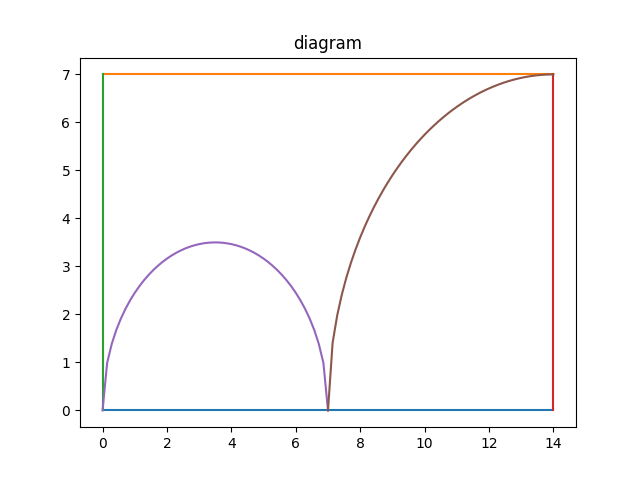
\includegraphics[scale = 0.5]{Figure_2.png}
    \caption{python programmed}
    \label{fig:my_label}
\end{figure}
\begin{center}
\textbf{Verification in python}    
\end{center}

\rule{\textwidth}{0.4pt}\\

\begin{figure}[h!]
    \centering
    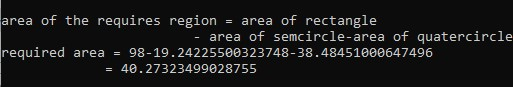
\includegraphics[scale = 0.6]{Figure_3.jpg}
    \caption{python}
    \label{fig:my_label}
\end{figure}

\end{document}
